\section{Autonomy Framework}

Our experiments are carried out on Boeing's Autonomy Testbed aircraft and simulation environment.  This testbed is used for the development of the collision avoidance LEC, the RTA architecture for ensuring safety, and for flight testing and demonstration.  

\subsection{Autonomy Testbed Aircraft}

%[MATT/JIM] Overview of the Boeing autonomy framework and aircraft used to demonstrate the collision avoidance neural network capability.

%Collision avoidance problem -- Strategic rather than tactical, avoidance flight plan must avoid intruder but return to original flight plan

%Limitations --  two-dimensional, lateral avoidance maneuvers, focus on single intruder

%Describe the safety requirements for collision avoidance.  Maybe reference DO-365. 

The Boeing Autonomy Testbed Aircraft is a Cessna Caravan 208B, tail number N208BX (Figure~\ref{fig:caravan}).  This platform is currently serving as a test bed for the DARPA Assured Autonomy program air domain experiments.  The Testbed is optionally piloted and serves as a means to demonstrate commercially viable technologies leading to autonomy.  It is a research and development vehicle able to operate in commercial airspace that is built on open-source middleware with in-house developed guidance and control technologies leveraged from across the Boeing enterprise.  The Testbed includes a full ``Iron Bird'' fixture for hardware-in-the-loop evaluation in which new autonomy technology can be fully integrated and tested before flight.  With this Testbed Boeing has demonstrated autonomy firsts including in-air detect and avoid, ADS-B transponder-based route planning for strategic avoidance, and fully autonomous ground taxi.

\begin{figure}
	\centering
	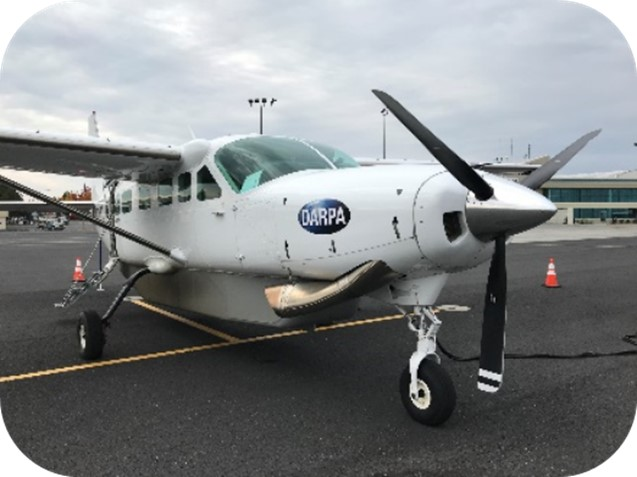
\includegraphics[width=\columnwidth]{figures/caravan.jpg}
	\caption{Boeing Autonomy Testbed Aircraft, Cessna Caravan 208B}
	\label{fig:caravan}
\end{figure}

Detect and avoid (DAA) mission operating and performance standards are defined in RTCA document DO-365 \cite{DO_365}.  The standard provides guidance for interactions of Unmanned Aircraft Systems (UAS) in the National Airspace System, requirements for safe operation of aircraft during encounters including separation distance minimums for remaining well clear of aircraft and avoiding mid-air collisions, and proper aircraft equipage to achieve safe detect and avoid operations.
The assurance challenge posed in our work focuses on the Autonomy Testbed aircraft flying in the vicinity of another ``intruder'' airplane, where the test flight software includes a Boeing-developed LEC to generate an avoidance flight plan for the Testbed to remain well clear of the intruder aircraft as defined in DO-365.  The underlying assurance technology montors the Boeing LEC in order to assess the avoidance trajectory from the LEC and guarantee safety. 

\begin{figure*}
	\centering
	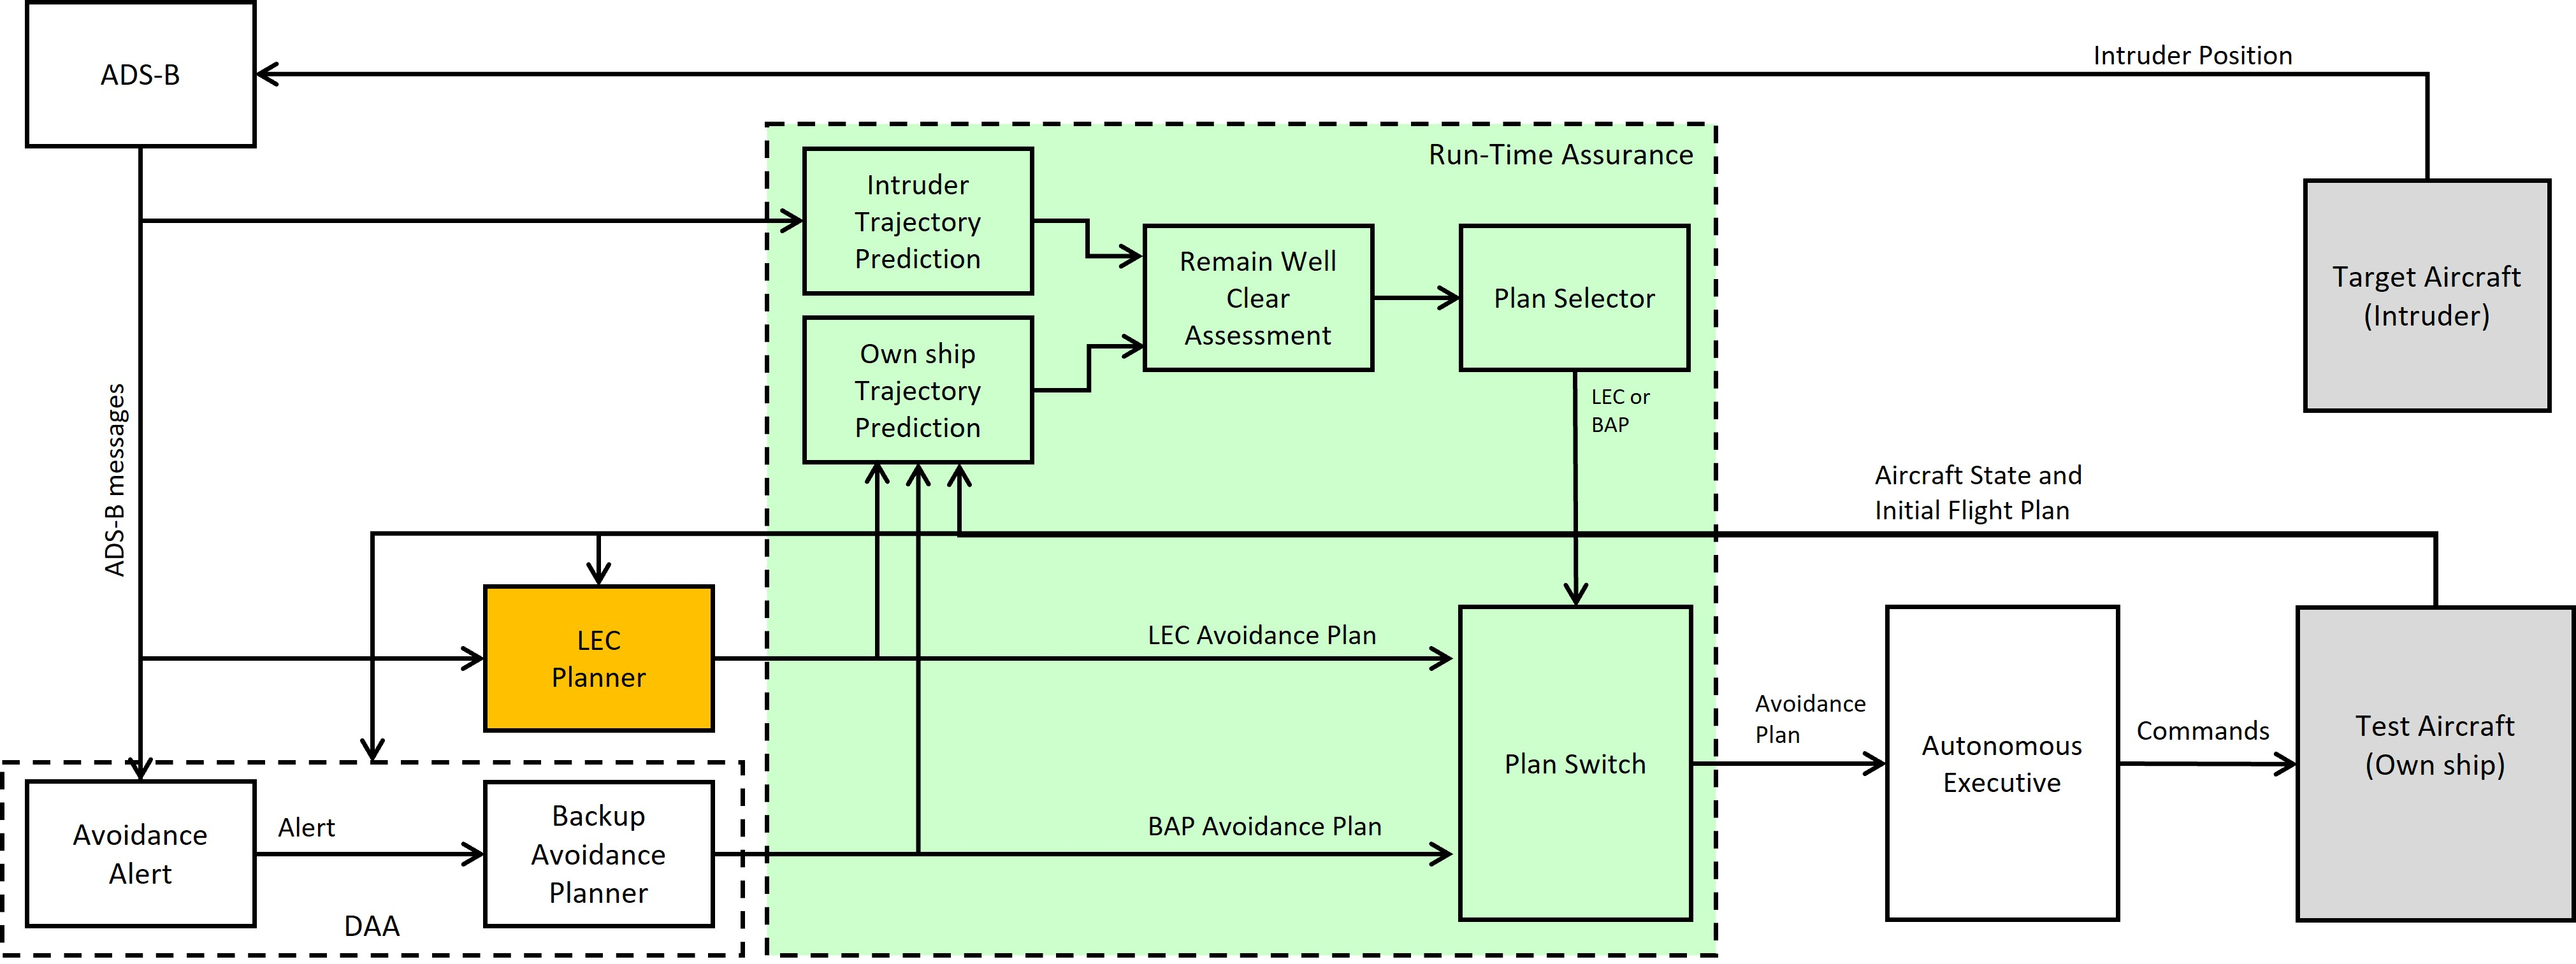
\includegraphics[width=\textwidth]{figures/rta-arch.jpg}
	\caption{Collision avoidance system on the autonomy testbed aircraft with run-time assurance components in green}
	\label{fig:rta-arch}
\end{figure*}

Figure~\ref{fig:rta-arch} shows a block diagram of the autonomy system framework as deployed on the Testbed aircraft.
System elements include: 
\begin{itemize}
\item ADS-B – The primary sensor for perceiving the airspace is the Automated Dependent Surveillance Broadcast (ADS-B) system providing detection information on  nearby aircraft (intruders) to the other system functions.
%\item ADS-B Tracker – Generates intruder track information from received ADS-B messages to the other system functions.
\item Avoidance Alerts – Evaluates potential future traffic conflicts and issues “alerts” to the Avoidance functions.  Assessment definition and requirements are specified in DO-365 MOPS for DAA System.
\item LEC Planner -- Neural network system trained offline through reinforcement learning to generate avoidance flight plans satisfying DAA requirements.  Training and operation is described in the following subsection.  
\item Backup Avoidance Planner – A trusted but less optimal backup planner that provides waypoint navigation paths to avoid airspace incursion.  Avoidance computation method is virtual predictive radar which is designed to provide maximum ``safe passage timed corridors.''  Avoidance path terminates back on the original flight plan.
\item Run-Time Assurance  – Run-time monitoring, predication, and assessment systems that guarantee the selection of a safe flight plan for the aircraft.  Operation and assurance are described in Sections \ref{sec:rta} and \ref{sec:assurance}.
\item Autonomous Executive – Constructs and manages execution of the vehicle flight plan and contains a function to ``splice in'' avoidance guidance waypoint plans into the original flight plan.
%\item Vehicle Manager – Executes flight path provided by AE including guidance and control for the vehicle.  The VM also sends commands and receives feedback from actuation system components.
%\item Actuators / Sensors – Carries out VMS flight control surface commands and provides positional feedback.
%\item Ownship State Estimation – Provides vehicle state information including position, altitude, and speed along with the vehicle inertial reference frame.
%\item Navigation Database – Reference database of aircraft parameters and airspace waypoints, terrain, airports, approaches, etc.  Used for route/avoidance planning purposes.
\end{itemize}


% Matt's section

\subsection{LEC Training with Reinforcement Learning}
%Description of LEC and RL, ROS integration

The LEC that generates the collsion avoidance flight plan is trained offline with a 
%In this work, the corrective maneuver for the avoidance is generated by a pre-computed solution -- 
Reinforcement Learning (RL) policy model. 
RL is a sequential policy optimization method that solves the task using the ``learning by doing'' concept and requires continuous data-rich interaction with the environment \cite{sutton2018reinforcement}. 
Our avoidance policy is trained on a surrogate task to provide the large number of interactions needed to achieve good performance. 
This surrogate environment developed by Boeing is a lightweight Python environment integrated with the OpenAI GYM framework \cite{brockman2016openai}.

The learned policy minimizes the risk of collision by providing continuous control commands in the surrogate environment. These commands are converted into a geometric trajectory (a sequence of waypoints) using the surrogate environment and a Robot Operating System (ROS) interface (Figure~\ref{fig:diagram}).

\begin{figure}[h]
	\centering
	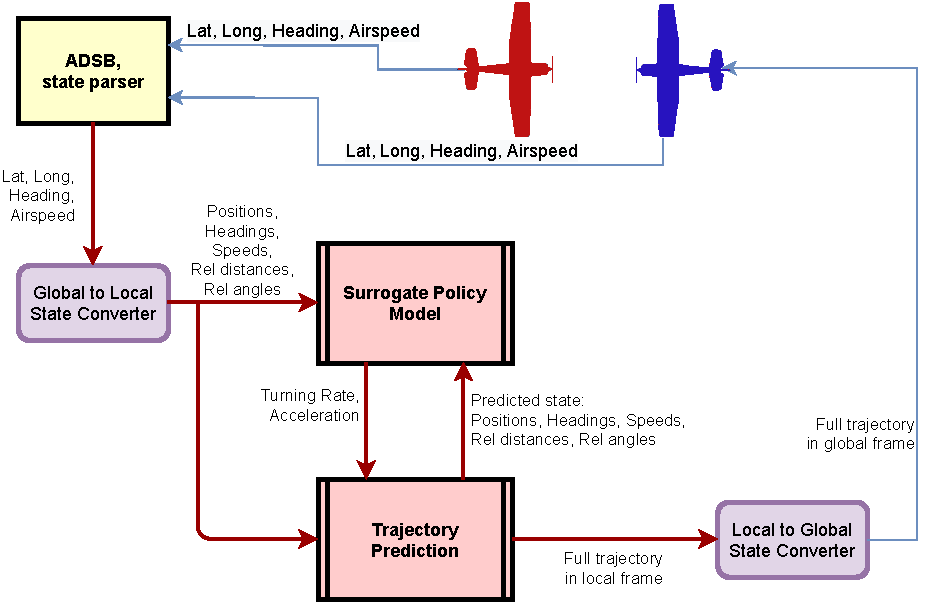
\includegraphics[width=\linewidth]{figures/system_overview.pdf}
	\caption{System diagram of the RL model-based conflict resolver.}
	\label{fig:diagram}
\end{figure}


Our surrogate environment is a simplified 2D obstacle avoidance problem that mimics the real task (air traffic conflict resolution). 
The environment simulates the movements of two aircraft on a 20x20 km square. The controlled Agent (representing the Autonomy Testbed Aircraft) has to go around the Intruder, provide minimal horizontal separation, and merge back to the next safe waypoint from the original route before the simulation ends.

%\begin{table}[h]
%	\centering
%	\begin{tabular}{||c | c | c||} 
%		\hline
%		Parameter & Range & Units \\
%		\hline
%		Time step $dT$ & 1.0  & sec \\
%		Max time $t_\text{MAX}$ & 300.0  & sec \\
%		Distance range & -10000 .. 10000  & m \\
%		Horizontal separation & 1000  & m \\
%		\hline
%	\end{tabular}
%	\caption{Surrogate environment simulation parameters.}
%	\label{tbl:sim_param}
%\end{table}


The surrogate dynamics imitate the dynamics of the Autonomy Testbed Aircraft.
%vehicle selected for the experiment -- a single-engine turboprop Cessna 208 Grand Caravan.
Both aircraft are represented by a simple dynamic model assuming massless kinematics and using Dubin's vehcile model for turn dynamics.
%\begin{itemize}
%	\item Dubin's vehicle model for turn dynamics
%	\item Mass-less kinematics model 
%	\end {itemize}
All the observation and control values are normalized to [-1..1] for the RL agent.
To make sure the agent generalizes the problem, we rewrap the observations and focus only on 
relative positions rather than absolute.  Repacked observations consumed by the agent:
	\begin{center}
		\begin{tabular}{|| c | c ||} 
			\hline
			heading & intruder heading\\
			airspeed & intruder airspeed\\
			distance to goal & distance to intruder\\
			tracking angle to goal & tracking angle to intruder\\
			\hline
		\end{tabular}
	\end{center}

\subsection{RL Policy Agent}

The RL policy agent learns the task by interacting with the simulation and iteratively updating the parameters of the policy model using Stochastic Gradient Descent (SGD) optimization. We approximate the policy with a multi-layered perceptron shown in Fig. \ref{fig:policy_model}.

\begin{figure}[h]
	\centering
	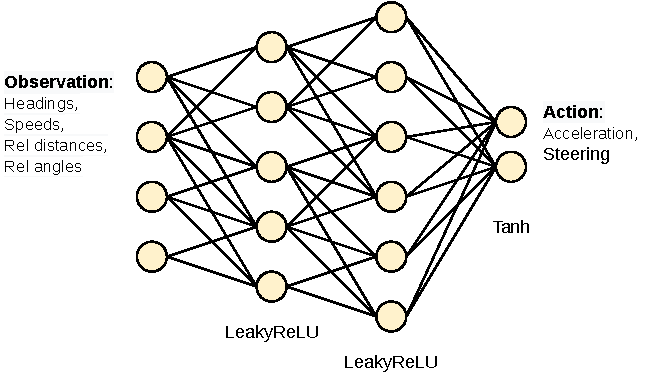
\includegraphics[width=0.8\columnwidth]{figures/model.pdf}
	\caption{Neural network function approximation used for the policy model consists of 2 hidden layers, 256 neurons each.}
	\label{fig:policy_model}
\end{figure}

To solve the optimization problem as Markov Decision Process (MDP), we refactor it into Markovian states $s$, transitions  $T(s' | s, a)$, and transition reward $R(s' | s, a)$. 
The state of the system (including both Agent and Intruder) is fully observable, assumes the perfect knowledge, and is enough to describe the Markovian state of the MDP system.
The state of the agent is described as
$$ s = \{ v_a, \psi_a, v_i, \psi_i, \beta_i, d_i, \beta_g, d_g \}$$

where 
$v_a$ is agent speed,
$\psi_a$ is agent heading,
$v_i$ is intruder speed,
$\psi_i$ is intruder heading,
$\beta_i$ is angle to intruder,
$d_i$ is distance to intruder,
$\beta_g$ is angle to goal, and
$d_g$ is distance to goal. 

The optimization is set to find the optimal policy $\pi^*(s)$ as a set of state-action mappings that maximizes the expected reward $V(s)$ \cite{sutton2018reinforcement}.
\begin{align} 
	\pi(s) &= P(a | s) \\
	\pi^*(s) &= \arg\max_{\pi} V^\pi (s) \\
	&= \arg\max_a \left( R(s,a) + \gamma T(s'|s,a) V(s') \right)
\end{align} 

The value of the state is the expected future reward accumulated over the trajectory and defined by the Bellman function as:
\begin{align}
	V(s) &=  \mathbb{E} [R | s, \pi] \\
	&= \sum_{s'} T(s'|s,a) \left( R(s'|s,a) + \gamma ( V(s')) \right) \\
	&=  R(s'|s,a) + \gamma \sum_{s'} T(s'|s,a) V^{\pi}(s') \\
	V^{*}(s) &= \max_{a} \left( R(s,a) + \gamma \sum_{s'} T(s'|s,a) V^{*}(s') \right)
\end{align}

The RL policy model is based on the Actor-Critic architecture that helps to improve the stability of the training \cite{sutton2018reinforcement}. The SGD-based update for Actor $\theta$ and Critic $w$ network is:
\begin{align}
	\delta &=  R_{t+1} +\gamma \hat V(s_{t+1},w) - \hat V(s_t,w) \\
	w &\leftarrow w + \alpha \delta \nabla \hat V (s, w) \\
	\theta &\leftarrow \theta + \alpha \delta \nabla \ln \pi (a|s, \theta)
\end{align} 

The core functionality of the RL agent incorporates the Stable Baselines library, a very reputable fork of OpenAI Baselines \cite{hill2018stable}. For the exploration policy and update steps, this work used the Proximal Policy Optimization (PPO) algorithm that becomes the state of the art in continuous-action agents \cite{schulman2017proximal}.


\subsection{LEC Integration on Testbed Aircraft}

\begin{figure}[h]
	\centering
	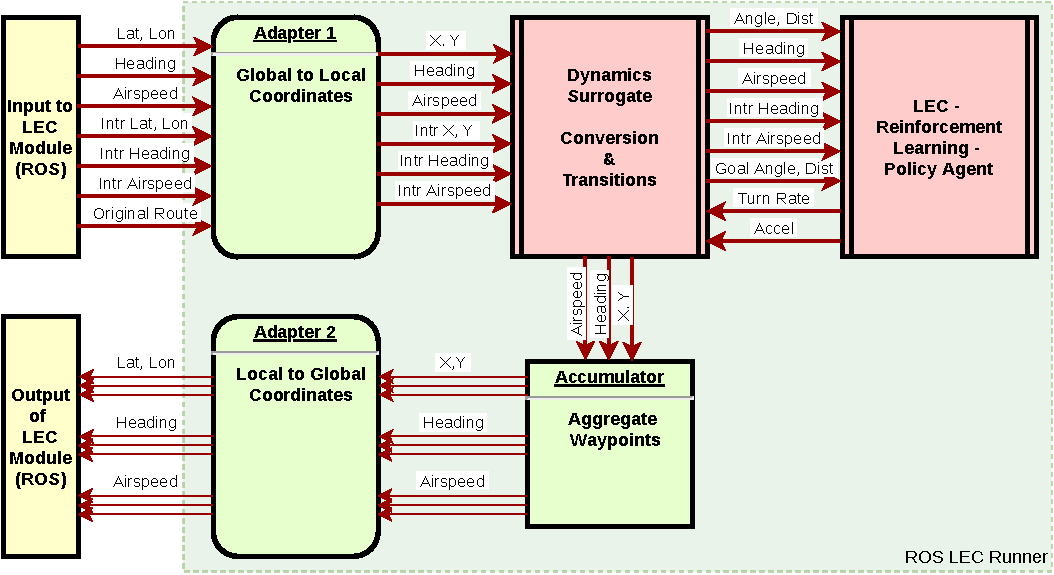
\includegraphics[width=\linewidth]{figures/cp25_ros.pdf}
	\caption{System diagram of the ROS-LEC node showing the integration of the learning-enabled component (LEC) to the aircraft using the ROS interface.}
	\label{fig:integration}
\end{figure}

System integration is done using the Robot Operating System (ROS) interface \cite{quigley2009ros}. This allows unifying the interfaces to the high-fidelity simulation and to the physical aircraft demonstrator.
The ROS-LEC Agent, shown in Figure~\ref{fig:integration}, aggregates data from different domains and provides important utilities to the system. Its job is designed as follows: 
\begin{itemize}
	\item receive and accumulate ROS messages regarding the own-ship state,
	Intruder's state, traffic alerts, GPS-SRS transformation data,
	\item translate ADS-B and GPS positioning data to local coordinate frame,
	\item extract the goal location from the original route,
	\item re-wrap the observations into the Agent-specific input format,
	\item iteratively run the Agent to get the corrective actions,
	\item iteratively run the surrogate environment to receive the transitions,
	\item form a corrective trajectory and check if the trajectory is good,
	\item translate the trajectory from local coordinate frame to global lat-long waypoints,
	\item publish the trajectory as a ROS message.
\end{itemize}

On an external request, the ROS-LEC agent generates a single avoidance flight plan and publishes it as ROS message. The flight plan consists of 20 waypoints in total. The last waypoint is taken from the original route, and 19 waypoints are generated by the policy. This allows linking the waypoints by a unique index and presere the indices of the original route.

These waypoints are spaced 20 seconds apart which provides a 400-second planning horizon. 
Because of the large time step between the waypoints, the policy and the surrogate have to be evaluated 20 times to make a single waypoint. The total response time of the system is below 60 msec for the complete trajectory.

%When needed to re-plan, the runner can be requested again. This architecture allows closed-loop corrections with an external run-time assurance monitor. The monitor keeps track of the accumulated transition error and either requests an updated avoidance plan or denies the operation switching to a back-up mode.
